\documentclass{article} % For LaTeX2e
\usepackage{nips13submit_e,times}
\usepackage{hyperref, color}
\usepackage{framed, graphicx}
\usepackage{subfigure}
\usepackage{kky}
\usepackage{url}
%\documentstyle[nips13submit_09,times,art10]{article} % For LaTeX 2.09


\title{Partitions for Efficient Inference on Graphical Models}
\author{
  Wenlu Hu\\
  Andrew ID: \texttt{wenluh} \\
  \texttt{wenlu@cmu.edu}
\And
  Kirthevasan Kandasamy\\
  Andrew ID: \texttt{kkandasa}\\
  \texttt{kandasamy@cmu.edu}
\And
  Joseph Tassarotti \\
  Andrew ID: \texttt{jtassaro} \\
  \texttt{jtassaro@andrew.cmu.edu}
%%\And
%%  Elara Willett \\
%%  Andrew ID: ehwillet \\
%%  \texttt{ehwillet@cs.cmu.edu}
}


\newcommand{\fix}{\marginpar{FIX}}
\newcommand{\new}{\marginpar{NEW}}
% \newcommand{\comment}[1]{\textcolor{magenta}{[#1]}}
\newcommand{\comment}[1]{}

\nipsfinalcopy % Uncomment for camera-ready version

\begin{document}
\maketitle

%\begin{abstract}
%abstract
%\end{abstract}t

%%%%%%%%%%%%%%%%%%%%%%%%%%%%%%%%%%%%%%%%% 

%\vspace{-0.25in}
\textbf{Note:} Many of the ideas in this paper, as well as significant portions of earlier drafts of the report, were contributed by Elara Willett, who is no longer enrolled in the course.


\section{Introduction} 

Probabilistic Graphical Models such as Bayesian Networks and Markov Random
Fields are ubiquitous in Machine Learning and Statistics. They allow us to
efficiently represent independence structures among variables in your
probability space. Gibbs Sampling, \cite{liu01mcmcscicomp} is a Markov Chain
based technique for drawing samples from such a graphical model. 
In Gibbs Sampling, we iteratively sample a subset of variables conditioned on
the other variables. We start with an arbitrary state and then run the Gibbs
Sampler for a specified burnin time after which the samples are collected.
As with most MCMC based methods, samples collected via Gibbs Sampling 
are correlated. Correlation between samples is an undesirable property
\cite{liu01mcmcscicomp} and affects our procedure in 2 ways. Firstly, the burn
in time will have to be large in order to make the ``sample quality''.
The correlation between samples depends on how slow the Markov Chain (MC) mixes.

A Naive Gibbs Sampler samples one variable at a time. This strategy is
computationally simple but usually there is significant correlation between
samples. Hence, we might need to run the Gibbs Sampler for several iterations.
A commonly used strategy is to group multiple
variables together in a Blocked Gibbs Sampler which improves the mixing rate of
the MC at the cost of increased computation for sampling from a more complex
conditional distribution at each step. Of course, making these blocks
arbitrarily complex is not an option since that would make sampling intractable
nullifying any gain obtained via a faster mixing time. The first figure of
Figure~\ref{fig:basefig} shows a simple graph followed by two ways to block the
variables in the graph for a Blocked Gibbs Sampler.

This leads to the interesting question as to whether we could develop an optimal
blocking strategy that gives us the best computational tradeoff between mixing
time and computational effort. Unfortunately studying this problem is not only
too difficult but even not well defined given that computational effort depends
on several factors such as the inference algorithm and the platform.
However, in the past some work has studied tree partitions
\cite{hamze2004fields, hamze2006information, rivasseau2005jungle}.
While Inference on a general graph is intractable, on trees algorithms such as
Belief Propagation 
converge exactly in a finite number of steps. Hence, in this project we will
adopt this strategy. For simplicity we assume that tree partitions provide a
good bargain in terms of computation. Hence, we will focus on obtaining the
``best'' tree-blocks of the graph.

To our knowledge, this problem has not studied extensively in Machine Learning
Literature -- current work only analyze simpler versions of the problem.
We aim to develop a method to work on arbitrary graphs. One of our important
novelties will be to take into consideration correlations between
variables in order to improve mixing time. While we can make no guarantees about
the results we will get, we are excited to be working on what we believe is an
interesting and relevant problem.


\newcommand{\gimgwidth}{0.9in}
\newcommand{\gimgspone}{0.3in}
\newcommand{\gimgsptwo}{0.04in}
\begin{figure}
\begin{center}
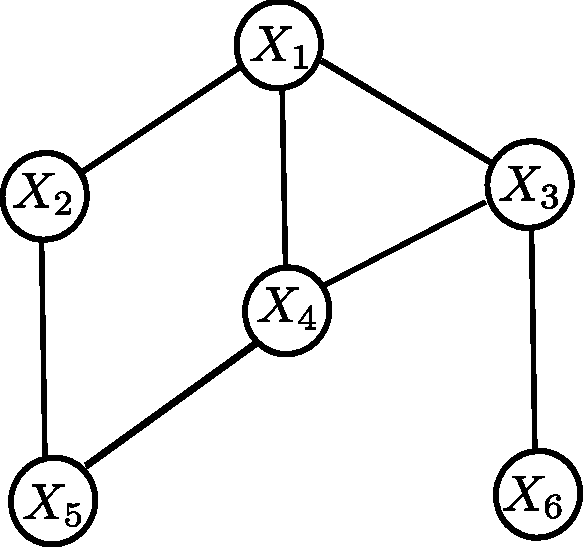
\includegraphics[width=\gimgwidth]{figures/orig_graph} \hspace{\gimgspone}
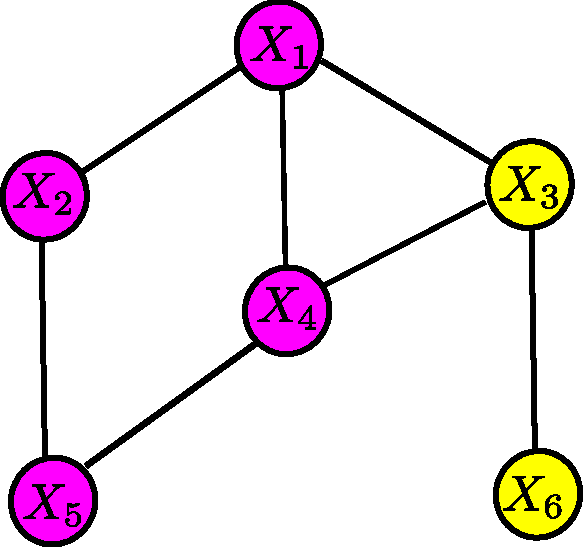
\includegraphics[width=\gimgwidth]{figures/bg2} \hspace{\gimgsptwo}
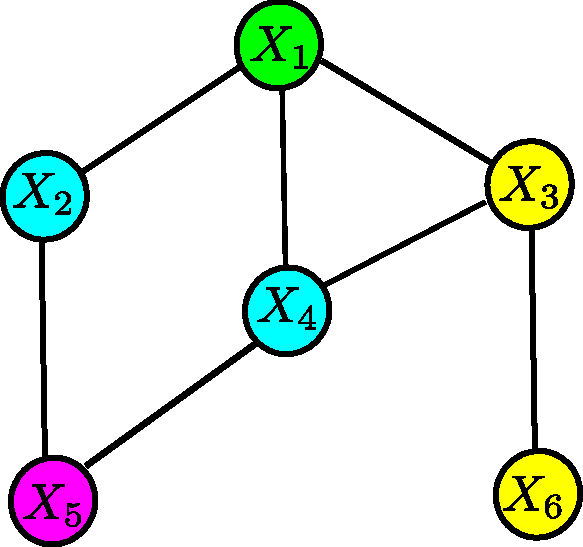
\includegraphics[width=\gimgwidth]{figures/bg3} \hspace{\gimgspone}
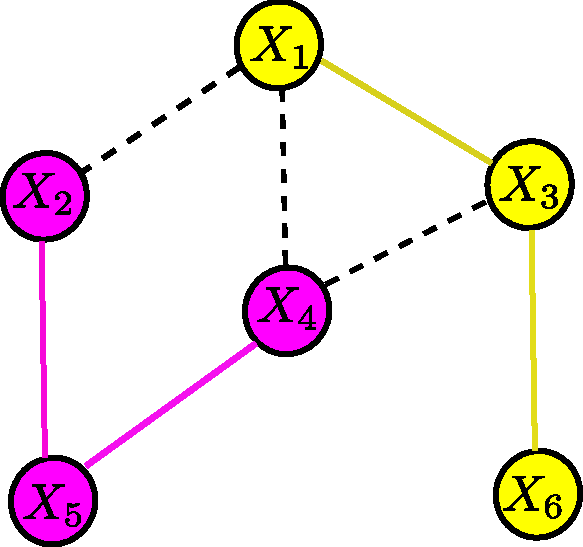
\includegraphics[width=\gimgwidth]{figures/tree1} \hspace{\gimgsptwo}
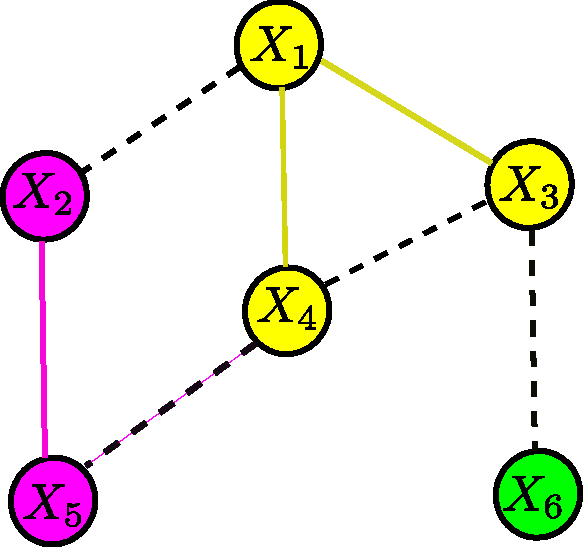
\includegraphics[width=\gimgwidth]{figures/tree2}
\end{center}
\caption{The first figure shows our original graph. The next two figures show to
blocking strategies for the variables in the graphs. The final two figures
show tree-blocking strategies. Trees are
computationally convenient than general blocks since inference on trees is
computationally easy.}
\label{fig:basefig}
\end{figure}

%%%%%%%%%%%%%%%%%%%%%%%%%%%%%%%%%%%%%%%%% 
\section{Related Work}
Finding partitions of a graph into trees for efficient inference has been
studied previously. 
In \cite{rivasseau2005jungle}, they  use a very simple heuristic which
aims to minimize the number of trees. 
In \cite{hamze2004fields, hamze2006information}, they
show that a Rao-Blackwellised
Estimator obtained via conditioning a two-tree partition of a Grid graph
outperforms a naive Gibbs sampler.

In order to study this problem methodically, we first need to ask ourselves what
characterizes faster mixing in a Markov Chain.
\cite{liu01mcmcscicomp,liu94covargibbs} argue that the mixing rate of a
Markov Chain is proportional to the norm of a ``Forward operator" $F$ defined on
a Hilbert Space of functionals of the variables. Hence a partitioning which has
smaller norm in the induced MC can be expected to mix faster.
\cite{hamze2006information, hamze2004fields} use these results to compare two
different partitions of a grid graph. They argue the superiority
of one over the other via the norm of the forward operator of the 
partition and back this conclusion with some experimental results.

%%%%%%%%%%%%%%%%%%%%%%%%%%%%%%%%%%%%%%%%% 
\section{Theory, Intuition and Insight to our Methods}
To set things up for the ensuing discussion, we begin with some results on
Markov Chains taken from \cite{liu01mcmcscicomp,liu94covargibbs}. We are given a
Markov Chain $ \Xii{1} \rightarrow \Xii{2} \rightarrow \dots \rightarrow \Xii{t}
\rightarrow \Xii{t+1} \rightarrow \dots $ with equilibrium distribution $\pi$.
We define the following set of functionals acting on our probability space
$L_0(\pi) = \{ h:\Omega \rightarrow \RR :\;\; \EE_{\pi} h(X) =
0, \;\; \VV_{\pi}h(X) < \infty \}$ and the inner product $\langle h, g \rangle =
\text{Covar}_\pi(h(X), g(X))$. It is straightforward to show that
$\big(L_0(\pi), \langle \cdot, \cdot \rangle \big)$ is a Hilbert Space (HS).
It can also be shown that the variance of a functional $h \in L_0(\pi)$ is its
squared norm: i.e. $\nbr{h}^2 = \VV_\pi(h(X))$.
On this Hilbert Space we define the following operator $F:L_0(\pi) \rightarrow
L_0(\pi)$, $ \,\; [Fh](\cdot) = \EE[h(\Xii{1}) | \Xii{0} = \cdot]$. In MC
literature $F$ is known as the Forward Operator. For reasons that will become
clear later we will call the norm of this operator $\nbr{F}$ the ``Mixing
Rate''. Using the Law of Total Variance we can show that $\nbr{F} \leq 1$.
Further, if the MC
is reversible (which is the case with a Gibbs Sampler) $F$ is self-adjoint and
hence the norm of the concatenation of $F$ satisfies $\nbr{F^n} = \nbr{F}^n$.
\cite{liu01mcmcscicomp} gives two results on $\nbr{F}$. The first of them is
characterizes faster mixing.

\begin{theorem}[\cite{liu01mcmcscicomp} Lemma 12.6.3]
Let $\Xii{0} \sim P^{(0)}$ where $P^{(0)}$ be an initial distribution satisfying
some regularity conditions. Let  $P^{(n)}$ denote $n^{th}$ step evolution of
$P^{(0)}$ obtained by passing it through the Markov Chain $n$ times. Let
$\EE^{(n)}$ be the expectation under $P^{(n)}$. Then,
\[
| \EE^{(n)} h(X) - \EE_\pi h(X) | \leq C \, \|F\|^n \, \|h\|.
\]
\end{theorem}

In brief, the above theorem says that $P^{(n)}$ will be closer to $\pi$ at a
rate determined by the mixing rate. The second result is on the variance of
samples collected after sufficient burn in.

\begin{theorem}[\cite{liu01mcmcscicomp} Theorem 12.7.2]
Let $\xii{1}, \dots, \xii{m}$ denote samples obtained from the Markov Chain
after sufficient mixing and $\bar{h}_m = \frac{1}{m} \sum_{j=1}^m h(\xii{j})$.
We then have the following CLT,
\begin{align*}
& \sqrt{m}(\bar{h}_m - \EE_\pi[h]) \overset{\Dcal}{\to} \Ncal(0, \sigma(h)^2)
\hspace{0.3in} \text{where} \\
& \sigma(h)^2 \leq \VV_\pi[h] \left( 1 + 2 \sum_{j=1}^\infty \nbr{F}^j \right)
\end{align*}
\end{theorem}

The above theorem says that the asymptotic variance of the samples collected
from a Gibbs Sampler increases monotonically with $\nbr{F}$. These results
convince us that suggest that keeping $\nbr{F}$ small in a Gibbs Sampler is
advantageous to obtaining higher quality samples. But how can this be done ?
\cite{liu01mcmcscicomp} also present the following equivalence between $\nbr{F}$
and the maximal correlation coefficient between samples collected from a MC.
\begin{equation}
\|F\| = \sup_{f,g} \text{Corr}(f(\Xii{t+1}), g(\Xii{t}))
\end{equation}
Here, $\Xii{t}, \Xii{t+1}$ are successive samples from a Markov Chain and the
supremum is over all functionals in $L_0(\pi)$.

While we do not have solid theoretical insight beyond this, we base our methods
on the following intuitions gained from above. In a Blocked Gibbs Sampler,
correlation between successive samples are induced by having correlation between
blocks. Hence, it pays to minimize the correlation between blocks. Equivalently,
we could try placing all strongly correlated variables in the same block. (We
note that this intuition is not new in the Machine Learning community, but we
were not able to find a precise theoretical formulation of this notion.) Now
given,
a graphical model, we now treat it as a weighted graph with the weights on edges
capturing the correlation between the variables at its ends. Our problem now is
to find tree partitions of this graph so as to maximize the intra-tree weights.

This leaves us with two challenges, The first 
is to weight any given graphical model using an
appropriate measure of correlation. Generally, this problem is nontrivial. We
discuss this issue and present our work around in
Section~\ref{sec:edgeweighting}. 
The second is to partition a graph into trees given such a weighting. 
This problem is NP-hard. In Section~\ref{sec:tpalgos}, we outline some heuristic
algorithms to achieve this objective.


%%%%%%%%%%%%%%%%%%%%%%%%%%%%%%%%%%%%%%%%% 
\section{Methods}

\subsection{Tree-Partitioning Algorithms}
\label{sec:tpalgos}

In order to employ blocked Gibbs sampling on our graphical model, we first partition the underlying graph into blocks. Inference on the blocks must be tractable, so we require the edges between vertices within a block to be a tree. We call the partitioning of a graph into blocks a splitting, which we define precisely as follows.

\noindent\textbf{$k$-Splitting:} Given a graph $G=(V,E)$, parameter $k$, and a weight function $w:E\rightarrow R$, output trees $T_1=(V_1,E_1),...,T_k=(V_k,E_k)$ such that:
\begin{enumerate}
\item For all $i,j\in[k]$, $V_i\cap V_j=\emptyset$, and $\cup_{i=1}^k V_i=V$.
\item For all $i\in[k]$, $u,v,\in V_i$, $\{u,v\}\in E_i$ if and only if $\{u,v\}\in E$.
\item For all $i\in[k]$, $u,v,\in V_i$, there is a unique path from $u$ to $v$ in $T_i$, i.e.~$T_i$ is a tree.
\end{enumerate}
Note that a tree is determined by its vertex set. So we can alternatively think of $k$-splitting as a coloring of the vertices, where the induced subgraph of each color is a tree. Also notice that the second criteria makes the $k$-splitting solution distinct from a spanning tree as show in Figure 1.
\begin{figure}
\begin{center}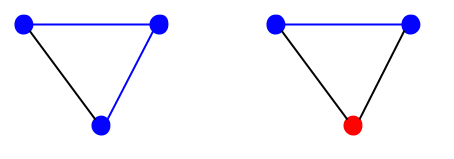
\includegraphics[scale=.5]{STvKS.png}\end{center}
\caption{The left graph depicts a spanning tree that is not a valid $1$-splitting since it violates criteria 2. The right graph depicts a $2$-splitting.}
\end{figure}

One possible measure of quality of a splitting is
\[
weight(T_1,...,T_k)=\sum_{i=1}^k\sum_{e\in E_i}w(e)
\]
Notice that in the case of a unit weight graph, the measure becomes
\[
weight(T_1,...,T_k)=\sum_{i=1}^k\sum_{e\in E_i}1=\sum_{i=1}^k|E_i|=n-k
\]
This tells us that in the unit weight case, the weight is maximized by minimizing the number of trees, $k$. In the design of our algorithms, the intermediate objectives we consider, which are believed correlate to fast convergence are 

\noindent\textbf{Unit-weight Objective:} Find a $k$-splitting for a small $k$.\\
\noindent\textbf{General-weight Objective:} Find a splitting with a small weight.

\subsection{Splitting Algorithms}%%%%%%
For a baseline, we consider the splitting algorithm from \cite{rivasseau2005jungle}. For their algorithm, they greedily grow trees favoring vertices of low degree. We present a slightly simplified version below. The priority queue is defined by
\noindent\textbf{compare(u,v)}: 
\[
|V\cap N(u)|>|V\cap N(v)| \iff u<v
\]
where $N(u)$ is the set of neighbor vertices to $u$, and $V$ is the set of uncolored vertices. Thus, we favor vertices with fewer uncolored neighbors.

\noindent Here we present a slightly simplified version of their algorithm.\\

\begin{framed}
\noindent\textbf{Greedy Tree Growing Algorithm \cite{rivasseau2005jungle}}
\begin{enumerate}
\item Initialize $i=0$ and $V$ to the vertex set.
\item While $V\neq\emptyset$
\begin{itemize}
\item Select $v\in V$
\item Start a new tree $T_i$ and a priority queue $Q_i$. Add $v$ to $Q_i$
\item While $Q_i\neq\emptyset$
\begin{itemize}
\item Pop $u$ from $Q_i$.
\item Initialize $neighborsInT=0$.
\item For all $v\in T_i$, if $u\in N(v)$, increment $neighborsInT$
\item If $neighborsInT\le1$,
\begin{itemize}
\item Add $u$ to $T_i$ and remove $v$ from $V$
\item Add $N(u)$ to $Q_i$.
\end{itemize}
\end{itemize}
\end{itemize}
\item Return $\{T_i\}$
\end{enumerate}
\end{framed}

Next, we present our contribution, the greedy edge selection algorithm. In our algorithm, we greedily select edges favoring edges of high correlation. To this end, we weight the edges by correlation.

\begin{framed}
\noindent\textbf{Greedy Edge Selection Algorithm}
\begin{enumerate}
\item Construct an ordered list of edges, $E$, with $E[0]$ being the highest weight edge. Edges are vertex pairs $(i,j)$.
\item Initialize an all-zero $n$-dimensional integer list $V$ of vertex colors. \\
($V[i]$ is the color of vertex $i$, and $V[i]=0$ means that vertex $i$ has not yet been colored.)
\item Initialize $n$ empty vertex sets: $T_1,...,T_n$\\
(Logically, $T_i$ is the set of vertices labeled with color $i$.)
\item Initialize $unusedColor=1$.
\item For each edge $e=(i,j)$ in $E$,
\begin{itemize}
\item If $V[i]=V[j]=0$,
\begin{itemize}
\item Set $V[i]=V[j]=unusedColor$
\item Add $i,j$ to $T_{unusedColor}$
\item Increment $unusedColor$ by $1$
\end{itemize}
\item Else if $V[i]=0$ and $V[j]\notin getOtherNeighborColors(\{i\}, e)$,
\begin{itemize}
\item Set $V[i]=V[j]$
\item Add $i$ to $T_{V[j]}$
\end{itemize}
\item Else if $V[j]=0$ and $V[i]\notin getOtherNeighborColors(\{j\}, e)$,
\begin{itemize}
\item Set $V[j]=V[i]$
\item Add $j$ to $T_{V[i]}$
\end{itemize}
\item Else if  $V[i]\neq 0$ and $V[j]\neq 0$ and $V[i]\notin getOtherNeighborColors(T_j, e)$,
\begin{itemize}
\item For each $k\in T_j$, set $V[k]=V[i]$
\item Set $T_i=T_i\cup T_j$
\item Set $T_j=\emptyset$
\end{itemize}
\item Otherwise do nothing
\end{itemize}
\item For each vertex $i$, if $V[i]=0$, set $V[i]=unusedColor$, $unusedColor++$
\item Output $\{T_j:T_j\neq\emptyset\}$
\end{enumerate}
\vspace{5mm}

\noindent\textbf{getOtherNeighborColors(S, e)}
\begin{enumerate}
\item Remove edge $e$ from the graph.
\item Initialize sets $neighbors=\emptyset$, $colors=\emptyset$
\item For each $i\in S$, $neighbors=neighbors\cup N(i)$
\item For each $i\in neighbors$, $colors=colors\cup V[i]$
\item Add $e$ back into the graph.
\item Return $colors$
\end{enumerate}
\end{framed}


\subsection{Edge Weighting}
\label{sec:edgeweighting}

We now turn to the problem of how we may weight these edges given a graphical
model. Generally, this problem is NP-hard. Even for the relatively simple class
of log-linear models it is not possible to estimate the correlations between two
variables directly. One technique is to sample from the model (say via a Gibbs
sampler) and estimate the correlation using the sample -- but this obviously
defeats the purpose since our very objective is to speed up the Gibbs Sampler.
This paints a rather bleak picture of the proposed strategy and at this point,
we unfortunately do not have a satisfying solution to it.

But in some cases this information could come via Expert knowledge. For example,
in large networks in computational biology etc. expert knowledge is already used
to group correlated variables together. In such situations our method is
applicable. Next there could be situations in which you repeat the same
inference task on a given graphical model under different observations. In such
situations we could run a Naive Gibbs sampler on a prototype observation and use
it to estimate the correlations. Then on subsequet inference procedures we use a
blocked gibbs sampler with tree blocks partitioned using the weights thus
learned. Even though observations do play an important role as when conditioned
any two variables could become more or less correlated - it is fair to assume
that they would be a reasoanable approximation to the actual correlations.


%%%%%%%%%%%%%%%%%%%%%%%%%%%%%%%%%%%%%%%%% 
\section{Experiments}

\subsection{Tree Splitting}%%%%%%

We have implemented both tree splitting algorithms described in the
Methods section.  We have run the algorithms on random-weight grid
graphs of various sizes. In these experiments we use random weights as
priorities for both algorithms. We have measured the total number of
trees generated, and the median tree size, which we believe are
correlated to fast convergence.

The results in figure~\ref{fig:treeResultsNumber} and
figure~\ref{fig:treeResultsMedian} show that our heuristic performs
much better than the splitting algorithm
from~\cite{rivasseau2005jungle}, when no other limits are imposed.
The leftmost data points in figure~\ref{fig:treeResultsNumber} show
that our heuristic generates half as many trees as the Greedy Tree
Growing algorithm. In figure~\ref{fig:treeResultsMedian},we also see
that median tree size for our Greedy Edge Selection algorithm is much
larger than the other algorithm. The median tree size for Greedy Tree
Growing algorithm is only 1, which means at least half of the trees
generated have only one vertex each.

Because sampling time can increase as trees grow in size, we are also
interested in the properties of the trees generated by the algorithms
when we impose a limit on the maximum tree size. However, as we impose
a tighter limit on the tree sizes, figure~\ref{fig:treeResultsNumber}
and figure~\ref{fig:treeResultsMedian} show that the Greedy Tree
Growing algorithm catches up with our heuristic. And as the limit
becomes as tight as 5, Greedy Tree Growing algorithm produces slightly
fewer trees and a larger median tree size. So our heuristic only
outperforms Greedy Tree Growing algorithm when the limit on maximum
tree size is no tighter than 10.


\begin{figure}
\centering
\subfigure[Total number of trees as maximum tree size limit
decreases.]{
	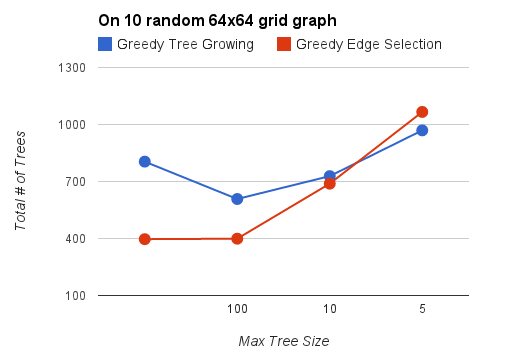
\includegraphics[width=0.48\textwidth]{figures/TotalTrees-Vs-MaxTreeSize} 
	\label{fig:treeResultsNumber}
}
\subfigure[Median tree size as maximum tree size limit decreases.]{
	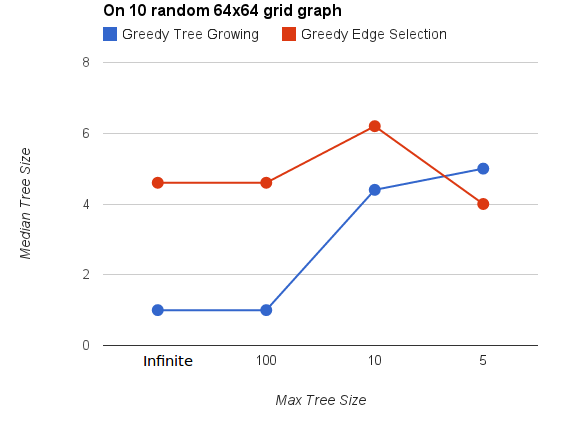
\includegraphics[width=0.48\textwidth]{figures/MedianTreeSize-Vs-MaxTreeSize}
	\label{fig:treeResultsMedian}
}
\caption{Comparing Greedy Edge Selection algorithm with Greedy Tree
Growing algorithm}
\end{figure}


\subsection{MCMC}%%%%%%

% We have been able to
% partially recreate some of the experiments in \cite{hamze2004fields}. We
% test only on Markov Networks with discrete states and use the Matlab library
% available at \cite{schmidt07ugm}.
% 
% The first experiment we recreated was Figure 6 in \cite{hamze2004fields}. We
% created a $10 \times 10$ grid graph and assigned $15$ possible states (with
% numeric value $1$ to $15$) to each node. We compare how fast each strategy mixes
% by running the sampler for $100$ iterations and studying how quickly a node
% converges to its expected value. We initialize all nodes at state $1$ and report
% the average results over $100$ trials.
% 
% We perform the above experiment on two different edge potentials to this grid
% graph. In the first we assign equal potential to all pairs of
% states for the neighboring nodes; i.e. the edge potential is a $15 \times 15$
% all ones matrix. Such a potential mixes fast and hence we can't really expect a
% Naive Gibbs sampler to perform badly. In fact, our experiments showed that the
% performance of all $3$ strategies were incomparable -- see
% Figure~\ref{fig:nodeprogunif}. Next we created random edge potentials but had
% high potentials for neighbors assuming similar states; i.e. the edge potential
% is a random matrix but with the diagonals being $5-6$ times larger than the off
% diagonals. Here, we found that the Two-Tree sampler outperforms the CheckerBoard
% and Naive Gibbs Samplers but the performance of the latter two were
% incomparable -- see Figure~\ref{fig:nodeprogrand}.
% 
% \begin{figure}
% \centering
%   \subfigure[Uniform Potentials]{
%   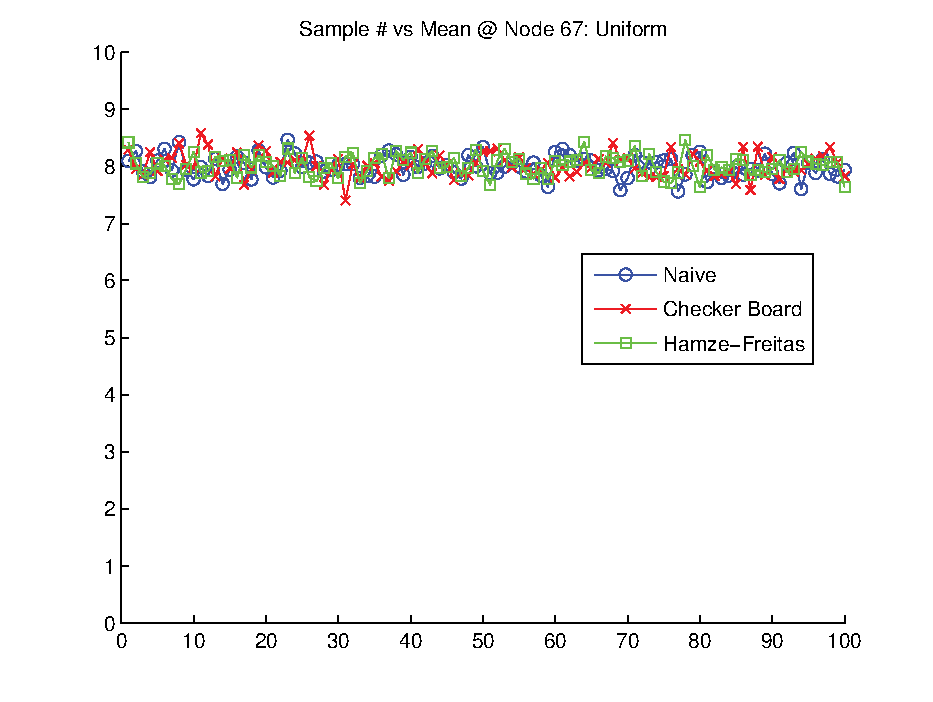
\includegraphics[width=2.5in]{figures/node_progress_uniform}
%   \label{fig:nodeprogunif}
%   }
%   \subfigure[Random Potentials]{
%   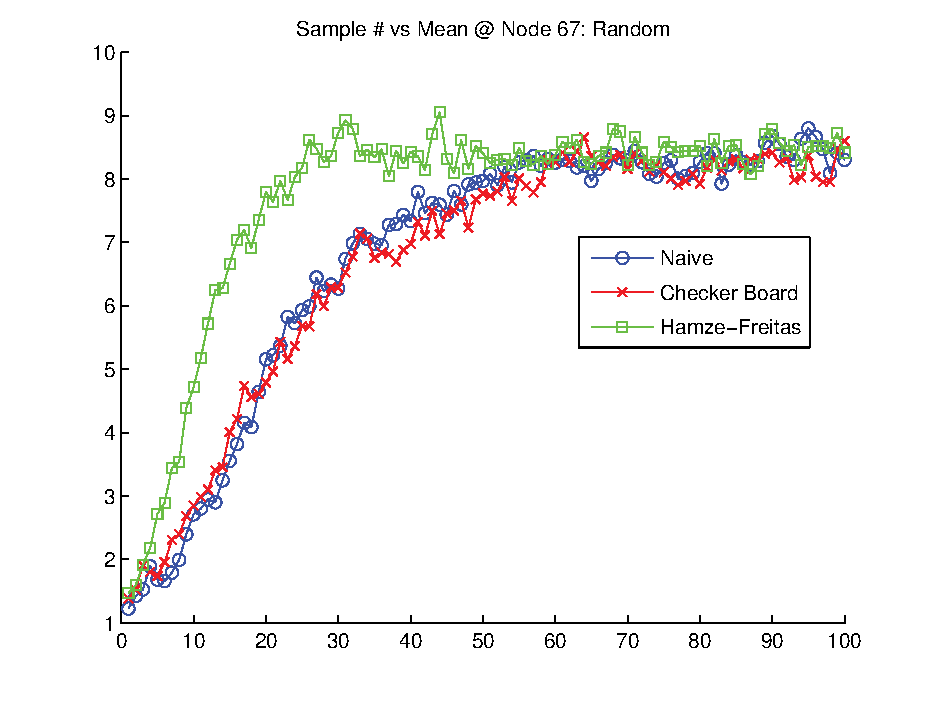
\includegraphics[width=2.5in]{figures/node_progress_random}
%   \label{fig:nodeprogrand}
%   }
% \caption[]{Comparison of the performance of the Naive Gibbs, CheckerBoard and
% Two-Tree Samplers in \cite{hamze2004fields}. Figure~\subref{fig:nodeprogunif} is
% for a grid graph with uniform edge potentials and
% Figure~\subref{fig:nodeprogrand} is for edge potentials with strong diagonals.}
% \label{fig:gibbsResults}
% \end{figure}
% 
% Note that the comparisons are based on the number of iterations and not
% computation time - which obviously is unfair to the Naive Gibbs Sampler. But
% we have not included a computation time based comparison for a few reasons - one
% of them being that our library has a fast $C++$ implementation for Naive Gibbs
% and a slow Matlab implementation of Tree Sampling. We intend to correct this in
% the future.


% partially recreate some of the experiments in \cite{hamze2004fields}. We
% test only on Markov Networks with discrete states and use the Matlab library
% available at \cite{schmidt07ugm}.

To compare these tree construction heuristics, we performed a variant of an
image reconstruction test found in~\cite{hamze2004fields}. In this experiment,
a $64\times64$ pixel test image was converted to grayscale, downsampled to a
4-bit colorspace, and then corrupted by randomly flipping the color of $25\%$
of the pixels. This problem was converted to an undirected graphical model with
a grid topology with one node for each pixel and isotropic edge potentials.  We
then tried to reconstruct the original image using different blocking strategies:

\begin{enumerate}
\item Naive Gibbs sampler -- no blocking
\item Checker Board blocks -- the network was divided up into two blocks in a checker board pattern
\item Hamze-Freitas Two Trees -- the network was divided up into two meshed trees
\item Trees generated using Greedy Tree algorithm -- we approximated correlations for the model by running 100 iterations of a separate Gibbs sampler. Tree sizes were limited to a maximum of 20.
\item Trees generated using Greedy Edge algorithm -- These used the same correlation estimates and tree size maximums.
\end{enumerate}

A visualization of the various blocks is shown in figure~\ref{fig:blockMaps}. The
first of these three strategies were compared in~\cite{hamze2004fields}.  Our
experiments were conducted using Schmidt's MATLAB library for undirected
graphical models~\cite{schmidt07ugm}, which we modified to add in the
Rao-Blackwellized tree sampler described in~\cite{hamze2004fields}. Each of the
five MCMC chains for each trial were started from the same initial point.

The results of this experiment are found in figure~\ref{fig:imageRecon}. The
relative performance gap between the Naive, Checker Board, and Two Trees are in
line with the results in~\cite{hamze2004fields}. The trees generated by the two
heuristics perform in between the Checker Board and the Two Trees, with the
Greedy Edge performing slightly better. Note that these experiments plot the
error rate versus the number of iterations of the Gibbs sampler, rather than
total computation time. In practice, the Two Trees strategy and the
automatically generated trees were considerably slower than the Checker Board
and the Naive Gibbs sampler, but this may be an artifact of the implementation
we used.

\begin{figure}
\begin{center}
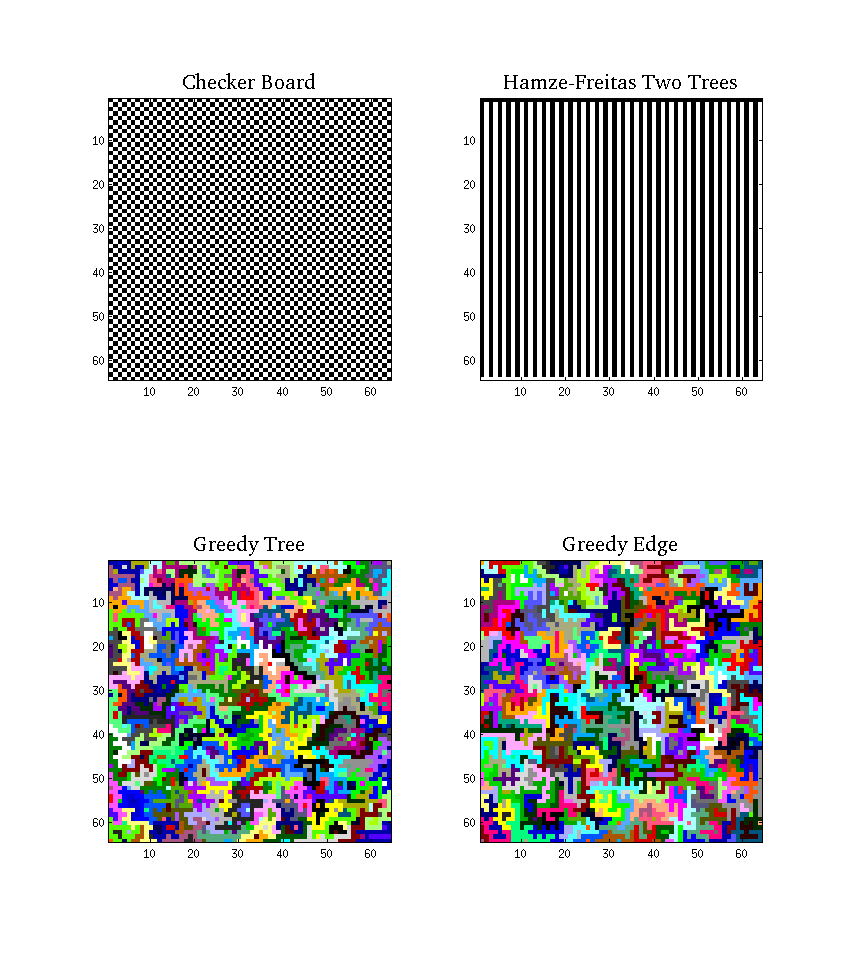
\includegraphics[width=3.5in]{figures/block_maps.png}
\vspace{-.5in}
\caption[]{Visualization of different blocks. Each color represents a separate block. The Greedy Edge and Greedy Tree blocks have a maximum tree size of $20$. Note that because trees are assigned colores randomly in this visualization, nearby trees may coincidentally be assigned a similar color, making it difficult to differentiate them.}
\label{fig:blockMaps}
\end{center}
\end{figure}

\begin{figure}
\begin{center}
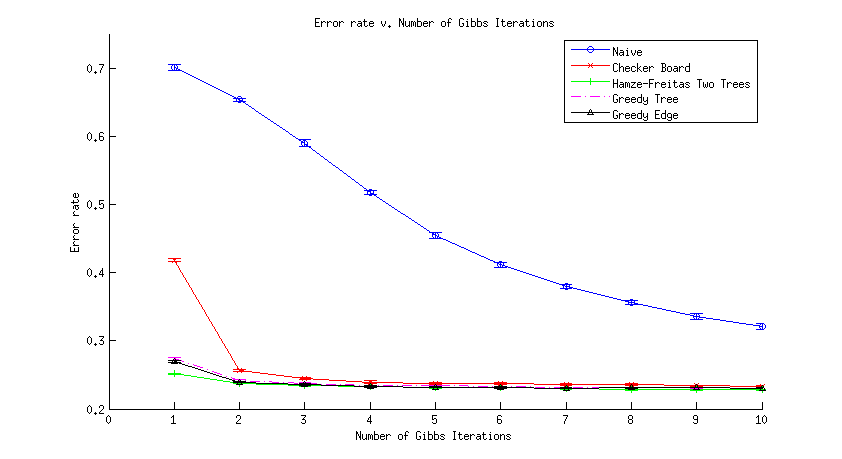
\includegraphics[width=5in]{figures/figure7_real}
\caption[]{Comparison of the performance of the Naive Gibbs, Checker Board, Hamze-Freitas Two-Trees, and automatically generated trees using the Rao-Blackwellized sampler on a vairant of the image reconstruction task from~\cite{hamze2004fields}.}
\label{fig:imageRecon}
\end{center}
\end{figure}

%%%%%%%%%%%%%%%%%%%%%%%%%%%%%%%%%%%%%%%%% 
\section{Conclusion}

We proposed a method to develop tree partitions for efficient blocked Gibbs
Samplers. The primary idea was to weight the edges of the graphical model
according to the correlation of the two variables and then convert it into a
tree partitioning problem. The objective in tree partitioning is to preserve the
high weight (highly correlated) edges within the trees and remove the low
weight edges. We outlined two heuristics to perform this which performed
reasonably well on our experiments.

Yet there are several points of concern in our work. The first is that there
is no straightforward way to estimate the correlation between two variables in a
graphical model without performing an actual inference task itself. At best, we
only know of some cheap ways to approximate this. However, trees partitioned
this way could still work well in practice. Second, while we did achieve faster
mixing in terms of iterations, when you factor in computation time the Naive
Gibbs Sampler beats tree sampling since it is computationally much cheaper. With
faster tree sampling implementations, we hope that we would be able to break
this barrier though.
Third, in many graphical models
especially sparse high dimensional ones - the tree structure encodes a
significant amount of the dependence structure. That is, two variables connected
by an edge in a graphical model are quite likely to be correlated themselves. In
such situations, it is not clear that our method would significantly outperform
(say) a random tree partitioning strategy.

\section*{Acknowledgements}
\label{sec:acknowledgement}
We thank Elara Willet for helping us with the Graph Theory element of
the project. She has worked closely with us in the first half
semester and has been really helpful.

\bibliographystyle{alpha} 
\bibliography{kky,final}     

%%%%%%%%%%%%%%%%%%%%%%%%%%%%%%%%%%%%%%%%% 
% \section*{APPENDIX}
% \noindent Work division so far:
% \begin{itemize}
% \item Wenlu- Implementing $k$-splitting algorithms.
% \item Kirthevasan- Implementing random graph generating, recreating experiments from \cite{hamze2006information}.
% \item Joseph- Implementing Rao-Blackwellized variant from \cite{hamze2006information} on top of UGM library, recreating experiments from \cite{hamze2006information}.
% \item Elara- Working on $k$-splitting algorithm design.
% \end{itemize}
% 
% Problem we have run into so far: our initial attempts to recreate the
% experiments from \cite{hamze2006information} without using the
% Rao-Blackwellized estimator they discuss turned-up negative results.  That is,
% the blocking strategies that they propose did not seem to have any advantage
% over Naive Gibbs Sampling when we did not use the Rao-Blackwell estimator.
% Later, we were able to confirm an effect using the RB estimator, and when
% working with non-uniform edge potentials, as we describe in the experimental
% section. We still need to do further work to understand the effects of the
% Rao-Blackwellization/non-uniform edge potentials.
% 
% \noindent Plan until the final:
% \begin{itemize}
% \item Run experiments using $k$-splitting algorithms.
% \item Implement a better greedy rule for unweighted graphs.
% \end{itemize}

\end{document}
